% comments start with "%"

% define document
\documentclass{article}[12pt] 

% margin spacing
\usepackage[a4paper, total={6in, 8in}]{geometry}

% package imports
\usepackage{hyperref}   % for hyperlinks
\usepackage{xcolor}     % for color options
\usepackage{amsmath}    % for math notation
\usepackage{graphicx}   % for graphics/image attachments
\usepackage{tikz}       % for drawing graphics
\usepackage{float}      % for figure positioning

% hyperref setup
\hypersetup{
    colorlinks=true,
    linkcolor=black,
    urlcolor=blue,
    pdfborderstyle={/S/U/W 1}
    }

% title setup
\title{Learning Notation: Introduction}
\author{
    Uppsala Pareto Seminars
    }
\date{}

% paragraph indent and spacing
\setlength{\parindent}{0pt}
\setlength{\parskip}{6pt}

\begin{document}
    
    \maketitle % create title
        
    \section{Welcome} % first section
        
        Welcome to the Learning Notation mathematics seminars! The seminars are organized by economics masters students in Pareto to discuss mathematics and economics in an informal setting.
        
        Some topics that we may venture are:
        
        % make a list
        \begin{itemize}
            
            \item
            proof techniques and set theory
            
            \item
            real analysis and advanced calculus
            
            \item
            differential equations and linear algebra
            
            \item
            probability theory
            
            \item
            complex numbers and their geometry
            
            \item
            and more!
            
        \end{itemize}
        
        The motivation of the seminars is to provide a forum where we can discuss and explore mathematics without the stress and obligations of an academic class. The hope is that we can discover some of the beauty and rigor of mathematical ideas together.\footnote{See \href{https://www.maa.org/external_archive/devlin/LockhartsLament.pdf}{A Mathematician's Lament}.}
        
        The name of the project, ``Learning Notation," comes from the idea that as daunting as mathematics can sometimes seem, it is just notation. If you understand the notation, you understand the math.
        
        
        We have a \href{https://www.overleaf.com/4797466783cszvmfmgsbct}{shared Overleaf project} where we collaborate on LaTex notes for the seminars. We also have a \href{https://discord.gg/Atv2jfRZnx}{Discord server} for announcements and discussion and a \href{https://docs.google.com/spreadsheets/d/1Ge9dVUt8bkdbZr03XvqzWJXrUtmdrix6Oo6ylrGNNsM/edit?usp=sharing}{Google Sheet} for scheduling.
    
    % start second section
    \section{How to use LaTeX}
        
        \href{https://www.overleaf.com/learn/latex/Learn_LaTeX_in_30_minutes}{Overleaf} has great resources for learning how to use \LaTeX. This section also serves as a quick primer on using math notation with LaTeX. See the \texttt{.tex} file for this document on Overleaf to see the LaTeX code and comments. % hello!
    
    % subsection under the second section
    \subsection{Writing math symbols}
        
        In LaTeX we can write in-line mathematical expressions alongside our text, for example: $\pi = 2\int_{-1}^{1}\sqrt{1 - x^2} \; dx \simeq 3.14159 $. \newline
        
        Using the \texttt{amsmath} package, we can also write single-line equations like so:
        \begin{equation}
            e^{i\pi} + 1 = 0.
        \end{equation}
        
        If we don't want the line numbers, we can use asterisks (*) to suppress them:
        \begin{equation*}
            1 + 2 = 3.
        \end{equation*}
    
        % use "\\" to start new line with
        % use "&" to align the lines
        We can also write multi-line equations.
        \begin{align}
            f(x) = a x^n, \; n \ge 2
            &\implies
            f'(x) = a n x^{n-1} \\  
            &\implies
            f''(x) = a n (n-1) x^{n-2}.
        \end{align}
        
        Again, if we don't want the line numbers, we can suppress them:
        \begin{align*}
            a x^2 + b x + c = 0
            & \implies x^2 + p x + q = 0,
            \quad p = \frac{b}{a}, \; q = \frac{c}{a}, \; a \ne 0,
            \\
            & \implies x^2 + p x = -q
            \\
            & \implies x^2 + p x + \left(\frac{p}{2}\right)^2
            = -q + \left(\frac{p}{2}\right)^2
            \\
            & \implies \left( x + \frac{p}{2} \right)^2
            = \frac{p^2}{4} - q
            \\
            & \implies x + \frac{p}{2}
            = \pm \sqrt{ \frac{p^2}{4} - q }
            \\
            & \implies x
            = -\frac{p}{2} \pm \sqrt{ \frac{p^2}{4} - q }.
        \end{align*}
    
    % start second subsection
    \subsection{Tables and graphics}
        
        With LaTeX we can create tables
        \begin{table}[H] % position table "here"
            \centering
            \begin{tabular}{|c||c|c|} % row text positioning
                \hline % horizontal line
                   & A   & B \\
                 \hline\hline % double lines
                 C & 0.1 & 0.2 \\
                 \hline
                 D & 0.3 & 0.4 \\
                 \hline % horizontal line
            \end{tabular}
            \caption{Example Table} % caption
        \end{table}
        
        and graphic figures
        \begin{figure}[H] % position graphic "here"
            \centering
            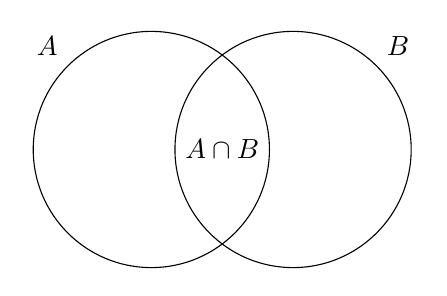
\begin{tikzpicture}
                % Set A
                \node [draw,
                    circle,
                    minimum size =3cm,
                    label={135:$A$}] (A) at (0,0){};
                % Set B
                \node [draw,
                    circle,
                    minimum size =3cm,
                    label={45:$B$}] (B) at (1.8,0){};
                % Set intersection label
                \node at (0.9,0) {$A\cap B$};
            \end{tikzpicture}
            \caption{Venn diagram}
        \end{figure}
        
        and also attach images as graphic figures.
        \begin{figure}[H]
            \centering
            % set width of graphic in-line with text
            \includegraphics[width=\textwidth]{attachments/0-pareto.jpg}
            \caption{Pareto logo}
        \end{figure}
        
        Document wise, \LaTeX{} can do pretty much anything. There's a lot to learn, but everything is just a Google search away.
        
\end{document}